% !TeX root = ../master.tex

\lecture{4}{2026-09-03}{Mikromekanik, Pt. I}

\section{Mikromekanik}
Grundlæggende er mikromekanik studiet af interaktionerne mellem fibrene og matrixen i en komposit.
Her arbejdes specielt med hvordan man kan forudsige egenskaberne for kompositter på baggrund af de indgående komponenter.
Det drejer sig specielt om
\begin{itemize}
  \item Youngs modul, $E$
  \item Poisson forhold, $\nu$
  \item Forskydningsmodul, $G$
  \item Termisk udvidelseskoefficient, $\alpha$
  \item Fugtig udvidelseskoefficient, $\beta$
\end{itemize}
Bemærk at de ovenstående ikke inkluderer styrker, da kompositstyrker er enormt svære at forudsige.


\begin{figure} [ht]
  \centering
  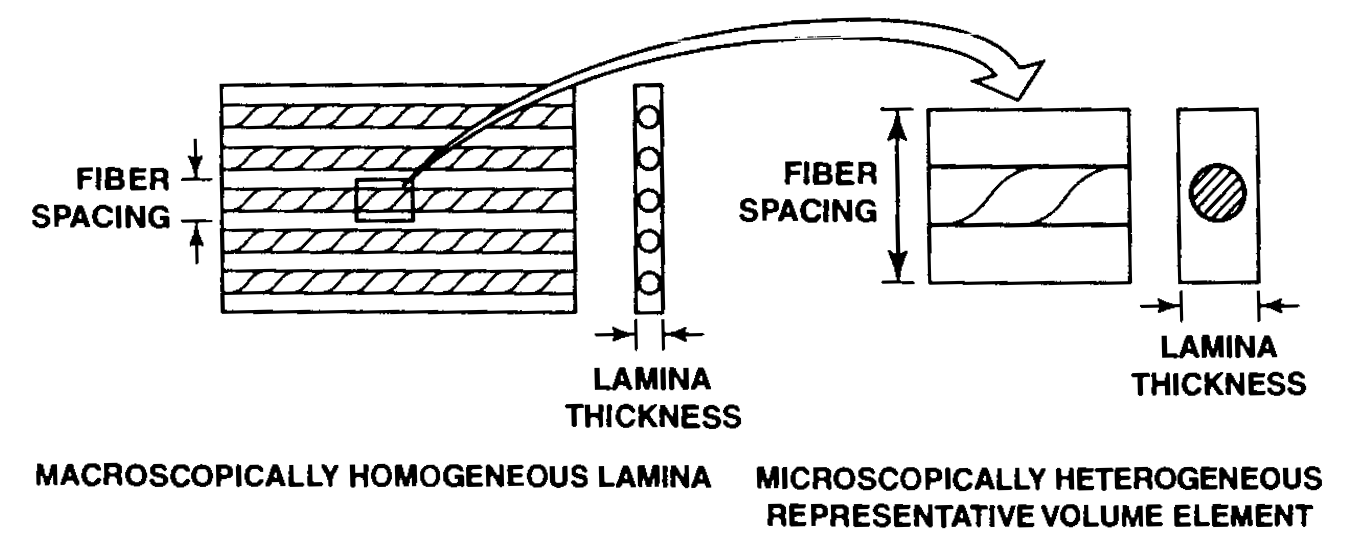
\includegraphics[width=0.7\linewidth]{./figures/jones_f_3_2.png}
  \caption{Repræsentativt volumenelement -- Lamina med unidirektionelle fibre, reproduceret fra \citepage{jones2021mechanicscompositematerials}{fig. 3--2}.}
  \label{fig:jones_f_3_2}
\end{figure}
På \Mref{fig:jones_f_3_2} ses en forstørret og idealiseret model af en lamina med unidirektionelle fibre.
Her arbejder vi grundlæggende med antagelserne i \Mref{tab:lamina-antagelser}:

\begin{table}[htbp]
  \centering
  \caption{Antagelser for lamina, fibre og matrix}
  \label{tab:lamina-antagelser}

  \begin{tabularx}{\textwidth}{
    |>{\raggedright\arraybackslash}X
    |>{\raggedright\arraybackslash}X
    |>{\raggedright\arraybackslash}X|
  }
    \hline

    \textbf{Lamina:}
    \begin{itemize}[leftmargin=*, nosep]
      \item Spændingsfri i ubelastet tilstand
      \item Lineær-elastisk
      \item Makroskopisk homogent
      \item Makroskopisk ortotropisk
    \end{itemize}

    &

    \textbf{Fibre:}
    \begin{itemize}[leftmargin=*, nosep]
      \item Homogene
      \item Lineær-elastiske
      \item Isotropiske
      \item Regulært fordelte
      \item Perfekt ensrettede
      \item Perfekt hæftede til matrixmaterialet
    \end{itemize}

    &

    \textbf{Matrix:}
    \begin{itemize}[leftmargin=*, nosep]
      \item Homogen
      \item Lineær-elastisk
      \item Isotropisk
      \item Luftboblefri
    \end{itemize}

    \\
    \hline
  \end{tabularx}
\end{table}

\subsection{Volumenfraktioner}
Vi arbejder typisk med to volumenfraktioner, navnligt fibervolumenfraktionen, $V_{\mathrm{f}}$, og matrixvolumenfraktionen, $V_{\mathrm{m}}$:
\begin{align*}
  V_{\mathrm{f}} &= \frac{\text{Fibervolumen}}{\text{Samlet Volumen}} \\
  V_{\mathrm{m}} &= \frac{\text{Matrixvolumen}}{\text{Samlet volumen}} \\
  V &= V_f + V_m = 1
.\end{align*}

\subsection{Stivheden langs fiberretningen}
Når en komposit belastes langs fiberretningen (1. retningen) antages at både fiberen og matrixen oplever den samme tøjning, $\epsilon_1 = \epsilon_{1\mathrm{m}} = \epsilon_{1\mathrm{t}}$.
Stivheden langs førsteretningen $E_1$ kan findes vha. den såkaldte rule of mixture:
\begin{equation*}
  E_1 = E_{\mathrm{f}} V_{\mathrm{f}} + E_{\mathrm{m}} V_{\mathrm{m}}
.\end{equation*}
Heraf bemærkes at det stiveste materiale på den måde vil være lastbærende.

\begin{figure} [ht]
  \centering
  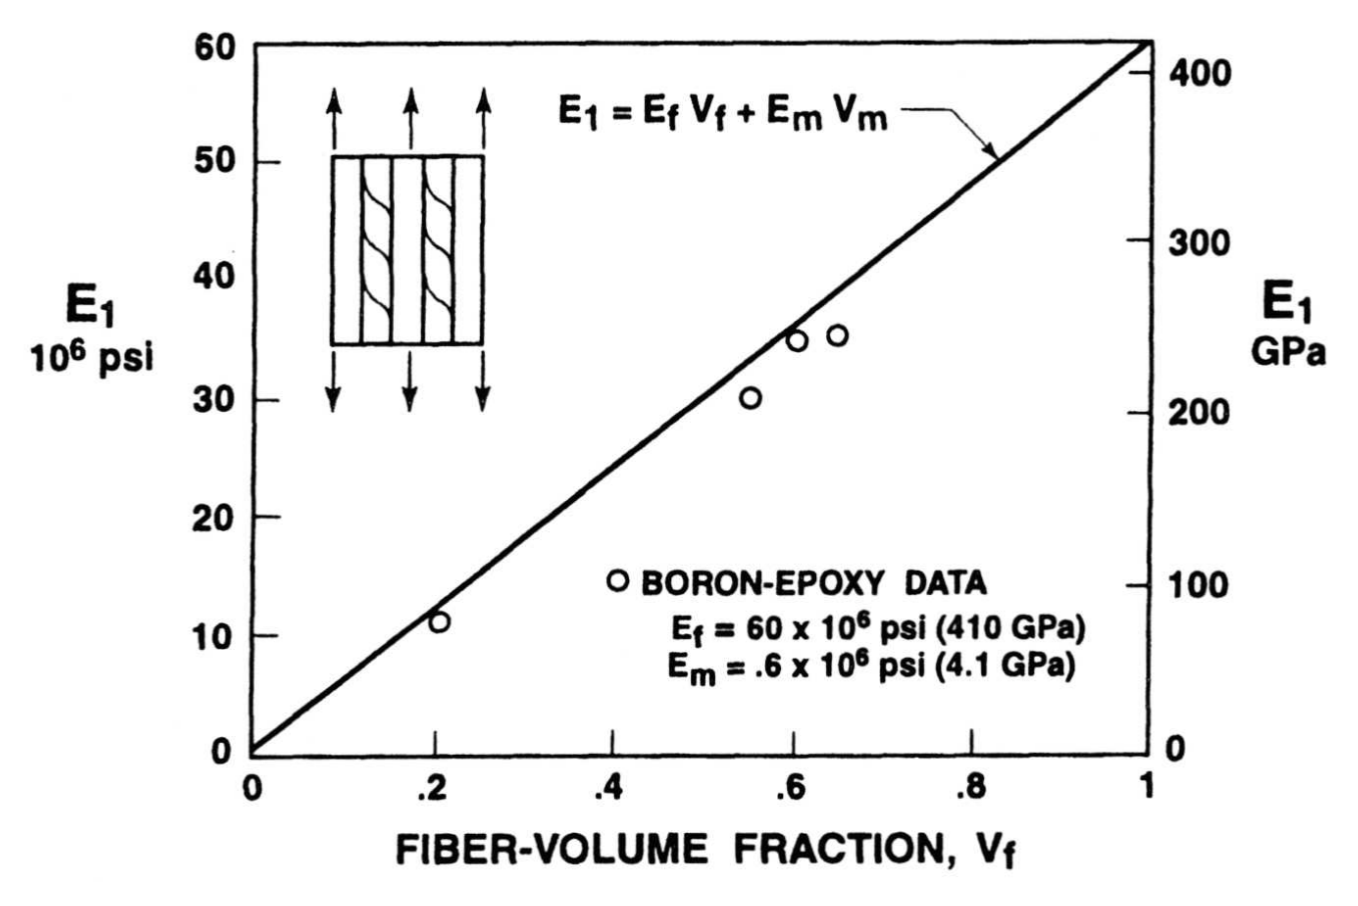
\includegraphics[width=0.6\linewidth]{./figures/jones_f_3_6.png}
  \caption{Variation i $E_1$ som følge af ændring af fibervolumenfraktion}
  \label{fig:jones_f_3_6}
\end{figure}
Af \mref{fig:jones_f_3_6} ses at materialegenskaberne for en komposit vil ligge på den rette linje mellem egenskaberne for de indgående materialer som følge af rule of mixture. 

\subsection{Stivheden på tværs af fiberretningen}
Når belastningen ligger i den transverse retning oplever både fiberen og matrixen det samme stress, $\sigma_{m2} = \sigma_{f2} = \sigma_{2}$. 
Hertil kan den inverse rule of mixture benyttes:
\begin{equation*}
  E_2 = \frac{E_f E_m}{E_m V_f + E_f V_m}
.\end{equation*}
Her bliver det mindst stive komponent begrænsende.

\begin{figure} [ht]
  \centering
  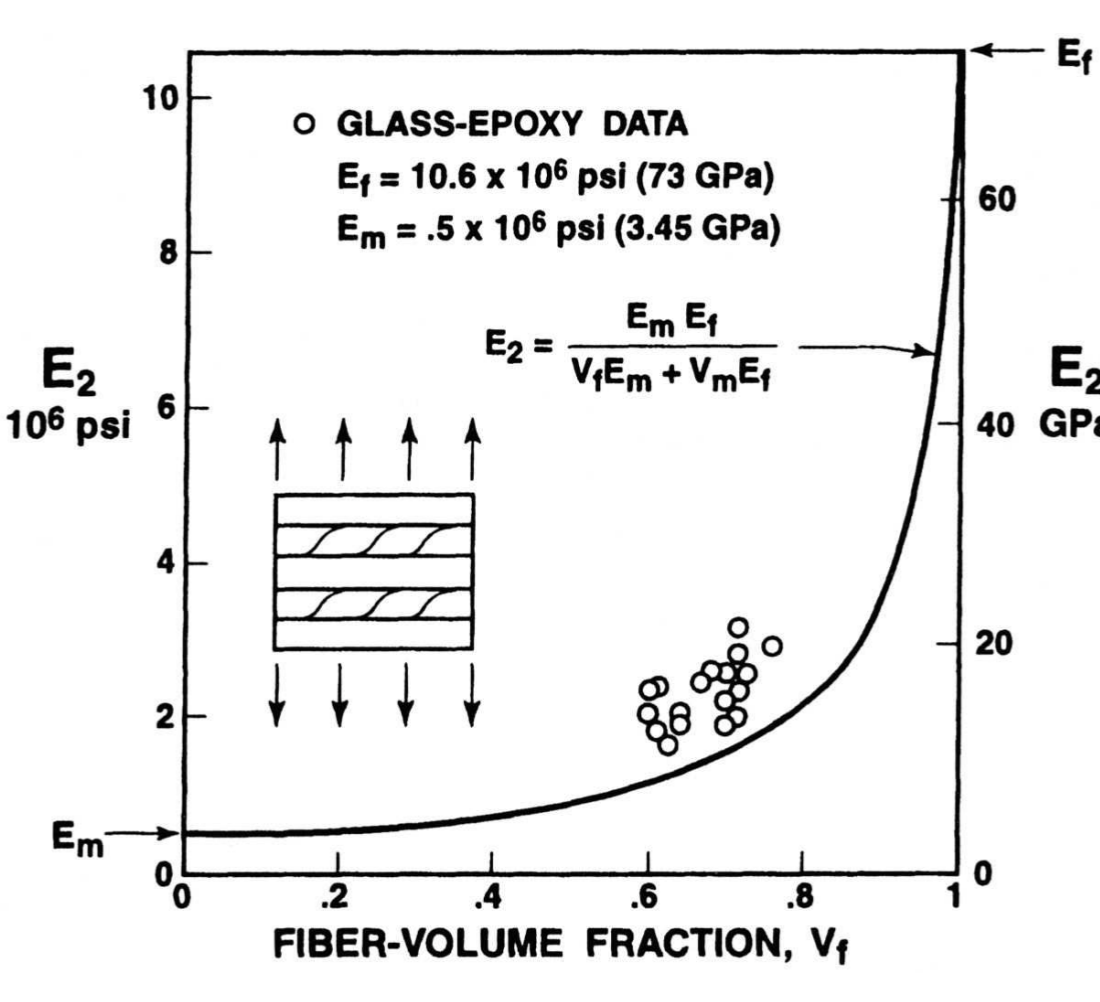
\includegraphics[width=0.6\linewidth]{./figures/jones_f_3_12.png}
  \caption{Forudsagt og målt $E_2$}
  \label{fig:jones_f_3_12}
\end{figure}
Som vist på \mref{fig:jones_f_3_12} er teorien mindre præcis her end hvad gjaldt for \mref{fig:jones_f_3_6}.
